
\setcounter{section}{1}
\renewcommand{\thesection}{\Asbuk{section}}
\sectioncentered*{ПРИЛОЖЕНИЕ А}
\addcontentsline{toc}{section}{Приложение А (обязательное) Исходный код программного средства}
\begin{center}
	\vspace{-1em}
	\textbf{(обязательное)}\\	
	\textbf{Исходный код программного средства}
\end{center}
\lstset{
	basicstyle=\footnotesize\ttfamily,
	breaklines=true, 
	language=C++,
	numbers=left,                    
	numbersep=5pt,
	tabsize=2,			
}
\lstinputlisting[caption=Исходный код класса DeltaBruteForce]{DeltaBruteForce.cpp}
\lstinputlisting[caption=Исходный код класса DeltaFromBorder]{DeltaFromBorder.cpp}
%\lstinputlisting[caption=Исходный код класса Mask]{Mask.cpp}

\setcounter{section}{2}
\setcounter{figure}{0}
\sectioncentered*{ПРИЛОЖЕНИЕ Б}
\addcontentsline{toc}{section}{Приложение Б (обязательное) Результаты исследования параметров порогового фильтра}
\begin{center}
	\vspace{-1em}
	\textbf{(обязательное)}\\	
	\textbf{Результаты исследования параметров порогового фильтра}
\end{center}
\begin{figure}[h]
	\centering
	\begin{subfigure}{0.45\textwidth}  
		\centering
		\includegraphics[width = \textwidth]{BF_ParamTestM1}
		\caption*{График для средней ошибки}
	\end{subfigure}    
	\begin{subfigure}{0.45\textwidth}  
		\centering
		\includegraphics[width = \textwidth]{BF_ParamTestM1den}        
		\caption*{График для плотности пикселей}
	\end{subfigure}
	\caption{Графики зависимостей для алгоритма использующего границы найденные оператором Робертса в качестве маски}
	\label{fig:PT_BF_M1}
\end{figure}

\begin{figure}[h]
	\centering
	\begin{subfigure}{0.45\textwidth}  
		\centering
		\includegraphics[width = \textwidth]{BF_ParamTestM2}
		\caption*{График для средней ошибки}
	\end{subfigure}    
	\begin{subfigure}{0.45\textwidth}  
		\centering
		\includegraphics[width = \textwidth]{BF_ParamTestM2den}        
		\caption*{График для плотности пикселей}
	\end{subfigure}
	\caption{Графики зависимостей для алгоритма использующего границы найденные оператором Собеля в качестве маски}
	\label{fig:PT_BF_M2}
\end{figure}

\begin{figure}[h]
	\centering
	\begin{subfigure}{0.45\textwidth}  
		\centering
		\includegraphics[width = \textwidth]{BF_ParamTestM3}
		\caption*{График для средней ошибки}
	\end{subfigure}    
	\begin{subfigure}{0.45\textwidth}  
		\centering
		\includegraphics[width = \textwidth]{BF_ParamTestM3den}        
		\caption*{График для плотности пикселей}
	\end{subfigure}
	\caption{Графики зависимостей для алгоритма использующего границы найденные оператором Превитта в качестве маски}
	\label{fig:PT_BF_M3}
\end{figure}


\begin{figure}[h]
	\centering
	\begin{subfigure}{0.45\textwidth}  
		\centering
		\includegraphics[width = \textwidth]{BO_ParamTestM1}
		\caption*{График для средней ошибки}
	\end{subfigure}    
	\begin{subfigure}{0.45\textwidth}  
		\centering
		\includegraphics[width = \textwidth]{BO_ParamTestM1den}        
		\caption*{График для плотности пикселей}
	\end{subfigure}
	\caption{Графики зависимостей для алгоритма основанного на поиске наилучшего наложения границ найденных оператором Робертса}
	\label{fig:PT_BO_M1}
\end{figure}
\begin{figure}[h]
\centering
\begin{subfigure}{0.45\textwidth}  
	\centering
	\includegraphics[width = \textwidth]{BO_ParamTestM2}
	\caption*{График для средней ошибки}
\end{subfigure}    
\begin{subfigure}{0.45\textwidth}  
	\centering
	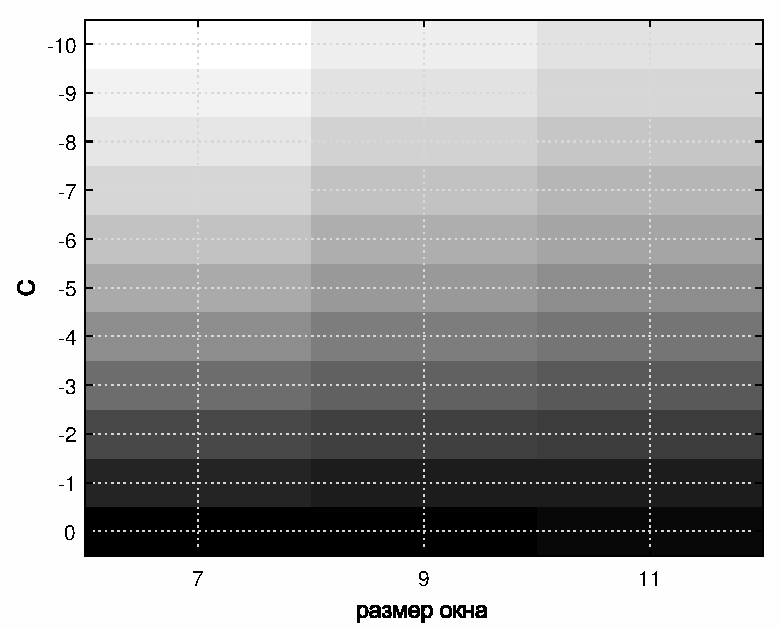
\includegraphics[width = \textwidth]{BO_ParamTestM2den}        
	\caption*{График для плотности пикселей}
\end{subfigure}
\caption{Графики зависимостей для алгоритма основанного на поиске наилучшего наложения границ найденных оператором Собеля}
\label{fig:PT_BO_M2}
\end{figure}
\begin{figure}[h]
\centering
\begin{subfigure}{0.45\textwidth}  
	\centering
	\includegraphics[width = \textwidth]{BO_ParamTestM3}
	\caption*{График для средней ошибки}
\end{subfigure}    
\begin{subfigure}{0.45\textwidth}  
	\centering
	\includegraphics[width = \textwidth]{BO_ParamTestM3den}        
	\caption*{График для плотности пикселей}
\end{subfigure}
\caption{Графики зависимостей для алгоритма основанного на поиске наилучшего наложения границ найденных оператором Преввита}
\label{fig:PT_BO_M3}
\end{figure}


\setcounter{section}{3}
\setcounter{figure}{0}
\sectioncentered*{ПРИЛОЖЕНИЕ В}
\addcontentsline{toc}{section}{Приложение В (обязательное) Пример изображения получаемого в результате работы программы}
\begin{center}
	\vspace{-1em}
	\textbf{(обязательное)}\\	
	\textbf{Пример изображения получаемого в результате работы программы}
\end{center}

\begin{figure}[h]
	\centering   
	\includegraphics[width=\textwidth,height=0.74\textheight,keepaspectratio ]{map} 
	\caption{Пример полученной карты}
	\label{fig:map}
\end{figure}

\begin{figure}[h]
	\centering   
	\includegraphics[width=\textwidth,height=0.74\textheight,keepaspectratio ]{mapCut} 
	\caption{Часть карты (увеличено)}
	\label{fig:mapCut}
\end{figure}